\begin{frame}{ビーム運動解析---BLC1-D5-BLC2}
  \begin{tabular}{cc}
    \begin{minipage}{0.5\hsize}
      \scriptsize
      \centering
      ビームの運動量解析はBLC1/2に挟まれた\\
      D5マグネットの輸送行列でBLC1とBLC2の\\
      トラックをつなぐことで行う。\\
      繋がれたトラックの$\chi^2/NDF<30$(赤線)\\をビームとみなす。\\
      BHDのヒットセグメントと\\$3\sigma$以内の相関があることを要求する。
    \end{minipage}

    \begin{minipage}{0.5\hsize}
      \begin{figure}
        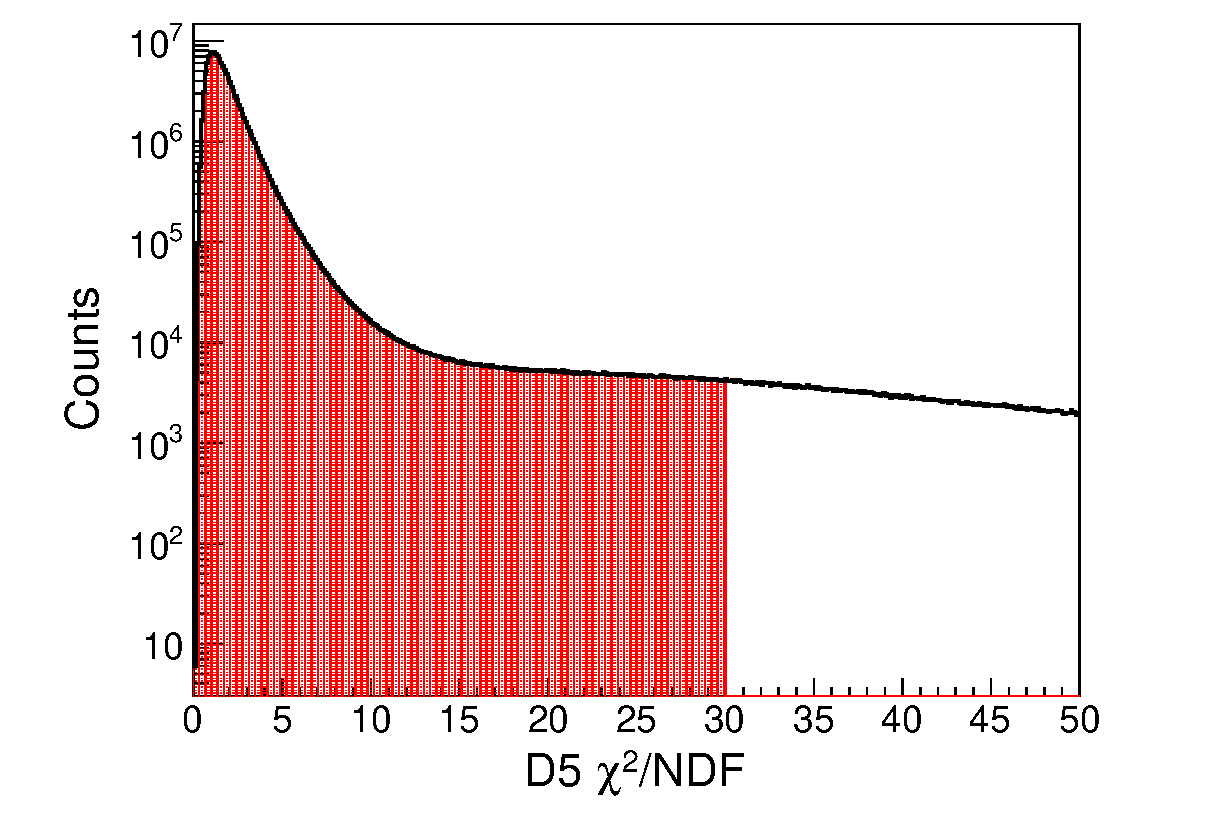
\includegraphics[width=4cm]{../pic/Run78/BL/D5_chi2.eps}
      \end{figure}
    \end{minipage}
  \end{tabular}

  \begin{tabular}{cc}
    \begin{minipage}{0.5\hsize}
      \begin{figure}
        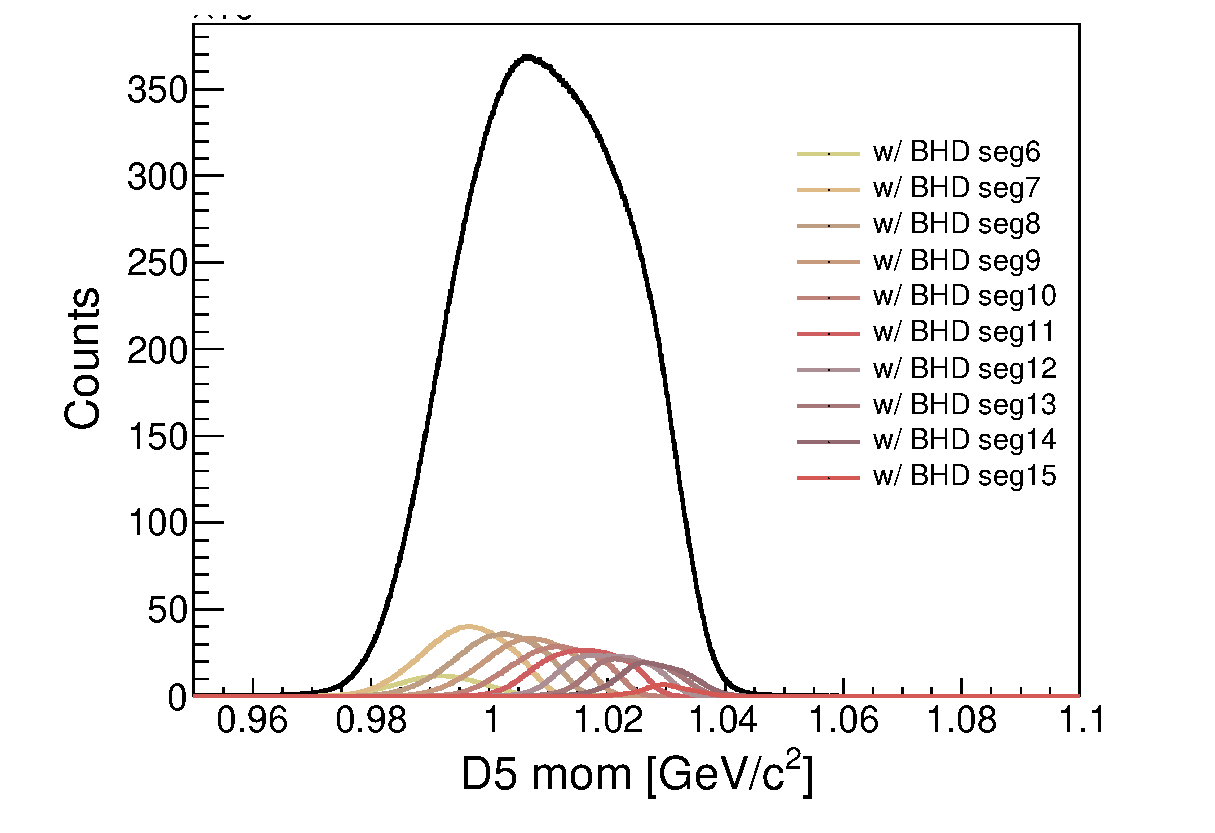
\includegraphics[width=4cm]{../pic/Run78/BL/D5_mom.eps}
      \end{figure}
    \end{minipage}

    \begin{minipage}{0.5\hsize}
      \begin{figure}
        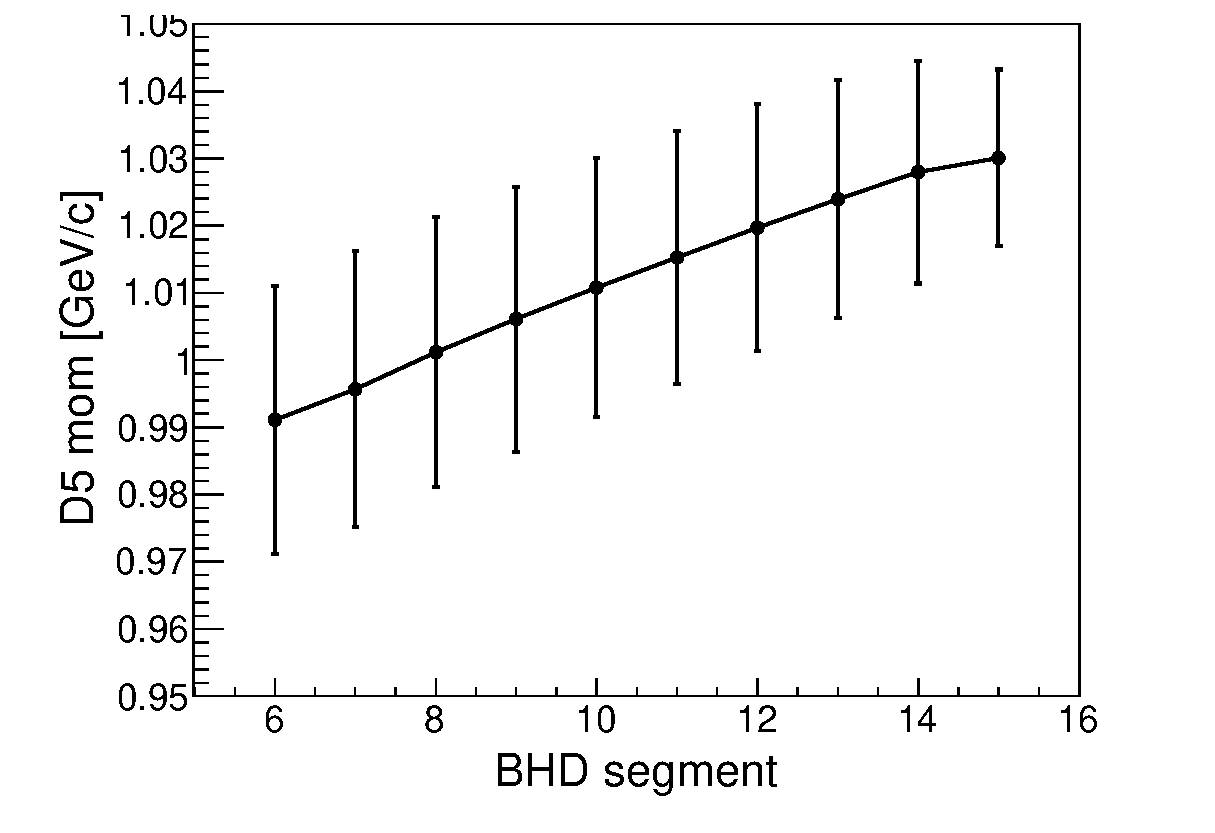
\includegraphics[width=4cm]{../pic/Run78/BL/D5_mom_BHDseg.eps}
      \end{figure}
    \end{minipage}
  \end{tabular}
  
  \centering
  \tiny
  左図は解析されたビームの運動量、色線はBHDが1ヒットのイベントでのBHDのヒットセグメントと運動量の関係\\
  右図は、各BHDセグメントとビーム運動量の中心地とビームとして受け入れる領域$3\sigma$を示している  
\end{frame}
